\documentclass[krantz2]{krantz}\usepackage{knitr}

\usepackage{color}

% \usepackage[scale=0.15,text={\copyright\ 2023 P. J. Aphalo, draft of \today}]{draftwatermark}

\usepackage{hologo}

\usepackage{csquotes}

\usepackage{graphicx}
\DeclareGraphicsExtensions{.jpg,.pdf,.png}

\usepackage{animate}

\usepackage[style=authoryear-comp,giveninits,sortcites,maxcitenames=2,%
    mincitenames=1,maxbibnames=10,minbibnames=10,backref,uniquename=mininit,%
    uniquelist=minyear,sortgiveninits=true,backend=biber]{biblatex}

\newcommand{\href}[2]{\emph{#2} (\url{#1})}

\usepackage{framed}

\usepackage{abbrev}
\usepackage{usingr}

\usepackage{imakeidx}

% for drawing flowcharts
\usepackage{tikz}
\usetikzlibrary{shapes.geometric,shapes.symbols,shapes.multipart,positioning,fit,arrows,matrix,backgrounds}
\tikzstyle{startstop} = [rectangle, rounded corners, minimum width=3cm, minimum height=1cm,text centered, draw=black]
\tikzstyle{io} = [trapezium, trapezium left angle=70, trapezium right angle=110, minimum width=3cm, minimum height=1cm, text centered, draw=black]
\tikzstyle{process} = [rectangle, minimum width=3cm, minimum height=1cm, text centered, draw=black]
%tight boxes
\tikzstyle{tprocess} = [rectangle, minimum width=2cm, minimum height=0.66cm, text centered, draw=black]
\tikzstyle{enclosure} = [rectangle, minimum width=3.4cm, minimum height=3cm, text centered, draw=black]
\tikzstyle{decision} = [diamond, aspect=2, minimum width=3cm, minimum height=1cm, text centered, draw=black]
\tikzstyle{arrow} = [thick,->,>=latex]

\tikzset{
 a/.style
  = {node distance=4em, text width=0.1em, minimum height=4em},
 b/.style
  = {rectangle, draw, fill=gray!10, node distance=4em, text width=6em,
     text centered, rounded corners, minimum height=4em, thick},
 c/.style
  = {circle, draw, dashed, fill=orange!10, inner sep = 0pt, node distance=4em, text width=6em,
     text centered, thick},
 cc/.style
  = {circle, draw, dashed, fill=orange!10, inner sep = 0pt, node distance=4em, text width=3em,
     text centered, thick},
 l/.style
  = {draw, -latex, ultra thick},
 aa/.style
  = {node distance=4em, text width=0em, minimum height=0.5ex},
 ll/.style
  = {draw, {open triangle 45} -, thick},
}

%\usepackage{polyglossia}
%\setdefaultlanguage{english}

% floats
\setcounter{topnumber}{3}
\setcounter{bottomnumber}{3}
\setcounter{totalnumber}{4}
\renewcommand{\topfraction}{0.90}
\renewcommand{\bottomfraction}{0.90}
\renewcommand{\textfraction}{0.10}
\renewcommand{\floatpagefraction}{0.70}
\renewcommand{\dbltopfraction}{0.90}
\renewcommand{\dblfloatpagefraction}{0.70}

% Include subsections as deepest nested in TOC
\setcounter{tocdepth}{2}
% Subsections as deepest numbered
\setcounter{secnumdepth}{2}

% ensure page numbers are aligned in TOC
\makeatletter
\renewcommand{\@pnumwidth}{2.05em}
\makeatother

\addbibresource{rbooks.bib}
\addbibresource{references.bib}

\makeindex[title=General Index]
\makeindex[name=rindex,title=Alphabetic Index of \Rlang Names]
\makeindex[name=rcatsidx,title=Index of \Rlang Names by Category]
\makeindex[name=faqindex,title=Frequently Asked Questions,columns=1]
\makeindex[name=cloudindex] % used for wordcloud
\IfFileExists{upquote.sty}{\usepackage{upquote}}{}
\begin{document}
\hyphenation{pro-cess-ing paren-the-ses spe-cif-ic au-thors in-ter-act-ed lim-it}

\title{\Huge{\fontseries{ub}\sffamily Learn R\\{\Large As a Language}}}

\author{Pedro J. Aphalo}

\date{Helsinki, \today}

% knitr setup

















\frontmatter

\maketitle

\newpage

\setcounter{page}{5} %previous pages will be reserved for frontmatter to be added in later.
\tableofcontents
\listoffigures
\listoftables



%\include{frontmatter/foreword}



\mainmatter












% !Rnw root = appendix.main.Rnw


\chapter{Base R: Adding New ``Words''}\label{chap:R:functions}

\begin{VF}
Computer Science is a science of abstraction---creating the right model for a problem and devising the appropriate mechanizable techniques to solve it.

\VA{Alfred V. Aho and Jeffrey D. Ullman}{\emph{Foundations of Computer Science}, 1992}\nocite{Aho1992}
\end{VF}

%\dictum[Alfred V. Aho, Jeffrey D. Ullman, \emph{Foundations of Computer Science}, Computer Science Press, 1992]{Computer Science is a science of abstraction---creating the right model for a problem and devising the appropriate mechanizable techniques to solve it.}\vskip2ex

\section{Aims of this chapter}

In earlier chapters we have only used base \Rlang features. In this chapter you will learn how to expand the range of features available. We will start by discussing how to define and use new functions, operators and classes. Later we will focus on using existing packages and touch briefly on how they work. We will not consider the important, but more advanced question of packaging functions and classes into new \Rlang packages.

\section{Defining functions and operators}\label{sec:script:functions}
\index{functions!defining new}\index{operators!defining new}

\emph{Abstraction} can be defined as separating the fundamental properties from the accidental ones. Say obtaining the mean from a given vector of numbers is an actual operation. There can be many such operations on different numeric vectors, each one a specific case. When we describe an algorithm for computing the mean from any numeric vector we have created the abstraction of \emph{mean}. In the same way, each time we separate operations from specific data we create a new abstraction. In this sense, functions are abstractions of operations or actions; they are like ``verbs'' describing actions separately from actors.

The main role of functions is that of providing an abstraction allowing us to avoid repeating blocks of code (groups of statements) applying the same operations on different data. The reasons to avoid repetition of similar blocks of code statements are that 1) if the algorithm or implementation needs to be revised---e.g., to fix a bug or error---it is best to make edits in a single place; 2) sooner or later pieces of repeated code can become different leading to inconsistencies and hard-to-track bugs; 3) abstraction and division of a problem into smaller chunks, greatly helps with keeping the code understandable to humans; 4) textual repetition makes the script file longer, and this makes debugging, commenting, etc., more tedious, and error prone.

How do we, in practice, avoid repeating bits of code? We write a function containing the statements that we would need to repeat, and later we \emph{call} (``use'') the function in their place. We have been calling \Rlang functions or operators in almost every example in this book; what we will next tackle is how to define new functions of our own.

We saw in section \ref{sec:script:compound:statement} on page \pageref{sec:script:compound:statement} a diagram of a compound statement. A function is a code statement, simple or compound, that is partly isolated from the enclosing environment. The \emph{function} abstraction relies on formal parameters working as placeholders for arguments within the function body. When the function is called (or ``used'') values are passed as arguments to the parameters, and used when executing the code within the function.

New functions and operators are defined using function \Rfunction{function()}, and saved like any other object in \Rlang by assignment to a variable name. In the example below, \code{x} and \code{y} are both formal parameters, or names used within the function for objects that will be supplied as \emph{arguments} when the function is called.

Function \code{my.prod()} has two formal parameters, \code{x} and \code{y}.

\begin{knitrout}\footnotesize
\definecolor{shadecolor}{rgb}{0.984, 0.984, 0.984}\color{fgcolor}\begin{kframe}
\begin{alltt}
\hlstd{fun1} \hlkwb{<-} \hlkwa{function}\hlstd{(}\hlkwc{x}\hlstd{,} \hlkwc{y}\hlstd{)\{x} \hlopt{*} \hlstd{y\}}
\end{alltt}
\end{kframe}
\end{knitrout}

When we call \code{fun1()} with \code{4} and \code{3} as arguments, the computation that takes place is \code{4 * 3} and the value returned is \code{12}. In this example it is printed, but we could have assigned it to a variable or used it in further computations within the calling statement.

\begin{knitrout}\footnotesize
\definecolor{shadecolor}{rgb}{0.984, 0.984, 0.984}\color{fgcolor}\begin{kframe}
\begin{alltt}
\hlkwd{fun1}\hlstd{(}\hlkwc{x} \hlstd{=} \hlnum{4}\hlstd{,} \hlkwc{y} \hlstd{=} \hlnum{3}\hlstd{)}
\end{alltt}
\begin{verbatim}
## [1] 12
\end{verbatim}
\end{kframe}
\end{knitrout}

\begin{playground}
What is the computation that takes places in this function call?

\begin{knitrout}\footnotesize
\definecolor{shadecolor}{rgb}{0.984, 0.984, 0.984}\color{fgcolor}\begin{kframe}
\begin{alltt}
\hlkwd{fun1}\hlstd{(}\hlkwc{x} \hlstd{=} \hlnum{10}\hlstd{,} \hlkwc{y} \hlstd{=} \hlnum{50}\hlstd{)}
\end{alltt}
\end{kframe}
\end{knitrout}
\end{playground}

\begin{warningbox}
Even though the statements within the function body do have access to the environment in which the function is called, it is safest to pass all input through the function parameters, and return all values to the caller. This ensures that the users of the function can treat it a black box with no side effects.
\end{warningbox}

\begin{figure}
  \centering
\begin{small}
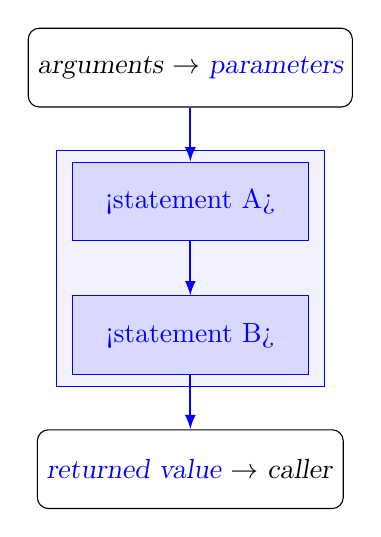
\begin{tikzpicture}[node distance=1.7cm]
\node (call) [startstop] {\textsl{arguments $\to$ \textcolor{blue}{parameters}}};
\node (enc) [enclosure, color = blue, fill = blue!5, below of=call, yshift=-0.85cm] {\ };
\node (stat1) [process, color = blue, fill = blue!15, below of=call] {\code{<statement A>}};
\node (stat2) [process, color = blue, fill = blue!15, below of=stat1] {\code{<statement B>}};
\node (return) [startstop, below of=stat2] {\textsl{\textcolor{blue}{returned  value} $\to$ caller}};
\draw [arrow, color = blue] (call) -- (stat1);
\draw [arrow, color = blue] (stat1) -- (stat2);
\draw [arrow, color = blue] (stat2) -- (return);
\end{tikzpicture}
\end{small}
  \caption[Diagram of function with no side effects]{Diagram of function with no side effects, seen as a compound code statement receiving its input as arguments passed to its formal parameters and returning an object or value to the statement from where it was called or run. The body of the function is represented by the filled box.}\label{fig:function:diagram}
\end{figure}

In \Rlang, statements within the function usually do not affect directly any variable defined outside the function, the result from the computation is returned as a value. The diagram in Figure \ref{fig:function:diagram} describes a function that has no \emph{side effects}, as it does not affect its environment, it only returns a value to the caller. A value on which the caller has full control. The statement that calls the function ``decides'' what to do with the value received from the function.

\begin{figure}
  \centering
\begin{small}
\begin{tikzpicture}[node distance=1.7cm]
\node (call) [startstop] {\textsl{arguments $\to$ \textcolor{blue}{parameters}}};
\node (enc) [enclosure, color = blue, fill = blue!5, below of=call, yshift=-0.85cm] {\ };
\node (stat1) [process, color = blue, fill = blue!15, below of=call] {\code{<statement A>}};
\node (sideeff) [process, color = black, fill = yellow!20, right of=stat2, xshift=3cm] {\textsl{\textcolor{blue}{side effect}}};
\node (stat2) [process, color = blue, fill = blue!15, below of=stat1] {\code{<statement B>}};
\node (return) [startstop, below of=stat2] {\textsl{\textcolor{blue}{returned  value} $\to$ caller}};
\draw [arrow, color = blue] (call) -- (stat1);
\draw [arrow, color = blue] (stat1) -- (stat2);
\draw [arrow, color = blue] (stat2) -- (sideeff);
\draw [arrow, color = blue] (stat2) -- (return);
\end{tikzpicture}
\end{small}
  \caption[Diagram of function with side effects]{Diagram of function as a compound code statement receiving its input as arguments passed to its formal parameters and returning an object or value to the statement from where it was called or run. The body of the function is represented by the box filled in blue, while the side effect of the code in the function directly outside is represented by the box filled in yellow.}\label{fig:function:side:effect:diagram}
\end{figure}

When a function has a side effect, the caller is no longer in full control (Figure \ref{fig:function:side:effect:diagram}). Side effects can be actions that do not alter any object in the calling code, like when a call to \Rfunction{print()} displays text or numbers. Side effects can also be an assignment that modifies an object in the caller's environment, such as assigning a new value to a variable in the caller's environment, i.e., ``outside the function''.

A function can return only one object, so when multiple results are produced they need to be collected into a single object. In many cases, lists are used to collect all the values to be returned into one \Rlang object. For example, model fit functions like \code{lm()}, discussed in section \ref{sec:stat:LM} on page \pageref{sec:stat:LM}, return lists with multiple heterogeneous members, plus ancillary information stored in several attributes. In the case on \Rfunction{lm()} the returned object's class is \Rclass{lm}, and its mode is \Rclass{list}.

\begin{playground}
When function \Rcontrol{return()} is called within a function, flow of execution within the function stops and the argument passed to \Rcontrol{return()} is the value returned by the function call. In contrast, if function \Rcontrol{return()} is not explicitly called, the value returned by the function call is that returned by the last statement \emph{executed} within the body of the function. Run these examples, and your own variations.

\label{chunck:print:funs}
\begin{knitrout}\footnotesize
\definecolor{shadecolor}{rgb}{0.984, 0.984, 0.984}\color{fgcolor}\begin{kframe}
\begin{alltt}
\hlstd{FN1} \hlkwb{<-} \hlkwa{function}\hlstd{(}\hlkwc{x}\hlstd{)} \hlkwd{print}\hlstd{(}\hlstr{"prn"}\hlstd{)}
\hlkwd{FN1}\hlstd{(}\hlstr{"arg"}\hlstd{)}
\hlstd{FN2} \hlkwb{<-} \hlkwa{function}\hlstd{(}\hlkwc{x}\hlstd{)\{}\hlkwd{print}\hlstd{(}\hlstr{"prn"}\hlstd{)}
                   \hlkwd{return}\hlstd{(x)\}}
\hlkwd{FN2}\hlstd{(}\hlstr{"arg"}\hlstd{)}
\hlstd{FN3} \hlkwb{<-} \hlkwa{function}\hlstd{(}\hlkwc{x}\hlstd{)\{}\hlkwd{return}\hlstd{(x)}
                   \hlkwd{print}\hlstd{(}\hlstr{"prn"}\hlstd{)\}}
\hlkwd{FN3}\hlstd{(}\hlstr{"arg"}\hlstd{)}
\hlstd{FN4} \hlkwb{<-} \hlkwa{function}\hlstd{(}\hlkwc{x}\hlstd{)\{}\hlkwd{return}\hlstd{()}
                   \hlkwd{print}\hlstd{(}\hlstr{"prn"}\hlstd{)\}}
\hlkwd{FN4}\hlstd{(}\hlstr{"arg"}\hlstd{)}
\hlstd{FN5} \hlkwb{<-} \hlkwa{function}\hlstd{(}\hlkwc{x}\hlstd{)\{}\hlkwd{return}\hlstd{(}\hlkwd{print}\hlstd{(x))}
                   \hlkwd{print}\hlstd{(}\hlstr{"prn"}\hlstd{)\}}
\hlkwd{FN5}\hlstd{(}\hlstr{"arg"}\hlstd{)}
\end{alltt}
\end{kframe}
\end{knitrout}
\end{playground}

In base \Rlang, arguments\index{functions!arguments} to functions are passed by copy. This is something important to remember. If code in a function's body modifies the value of a parameter (the placeholder for an argument), its value outside the function is not affected, e.g., if the argument passed was a variable.

\begin{knitrout}\footnotesize
\definecolor{shadecolor}{rgb}{0.984, 0.984, 0.984}\color{fgcolor}\begin{kframe}
\begin{alltt}
\hlstd{fn2} \hlkwb{<-} \hlkwa{function}\hlstd{(}\hlkwc{x}\hlstd{)\{x} \hlkwb{<-} \hlnum{99}\hlstd{\}}
\hlstd{a} \hlkwb{<-} \hlnum{1}
\hlkwd{fn2}\hlstd{(a)}
\hlstd{a}
\end{alltt}
\begin{verbatim}
## [1] 1
\end{verbatim}
\end{kframe}
\end{knitrout}

\begin{warningbox}
In some other computer languages, arguments can be passed by reference, meaning that assignments to a formal parameter within the body of the function are back-referenced to the argument and modify it. It is possible to imitate such behavior in \Rlang using some language trickery and consequently, occasionally functions in \Rlang use this approach.
\end{warningbox}

Functions have their own \emph{scope}. Any new variables created by normal assignment within the body of a function are visible only within the body of the function and are destroyed when the function returns from the call. In normal use, functions in \Rlang do not affect their environment through side effects.

\subsection{Scope of names}
\index{names and scoping}\index{scoping rules}\index{namespaces}
Scoping in \Rlang is implemented using \emph{environments} and \emph{name spaces}. We can think of environments as having a boundary with asymmetric visibility. The code within a function runs in its own environment, in isolation from the calling environment in relation to assignments, but the values stored in objects in the calling environment can be retrieved. This protects from unintentional side effects by making difficult to overwrite object definitions in the calling environment. It is possible to override this protection with operator \Roperator{<<-} or with function \Rfunction{assign()}. When used, assignment as side effects, can make the code much more difficult to read and debug, so its best to avoid them.

The visibility of names is determined by the \emph{scoping rules} of a language. The clearest, but not the only situation when scoping rules matter, is when objects with the same name coexist. In such a situation one will be accessible by its unqualified name and the other hidden but possibly accessible by qualifying the name with the namespace where it is defined.

As the \Rlang language has few reserved words for which no redefinition is allowed, we should take care not to accidentally reuse names that are part of language. For example \code{pi} is a constant defined in \Rlang with the value of the mathematical constant $\pi$. If we use the same name for one of our variables, the original definition becomes hidden.

\begin{knitrout}\footnotesize
\definecolor{shadecolor}{rgb}{0.984, 0.984, 0.984}\color{fgcolor}\begin{kframe}
\begin{alltt}
\hlstd{pi}
\end{alltt}
\begin{verbatim}
## [1] 3.141593
\end{verbatim}
\begin{alltt}
\hlstd{pi} \hlkwb{<-} \hlstr{"apple pie"}
\hlstd{pi}
\end{alltt}
\begin{verbatim}
## [1] "apple pie"
\end{verbatim}
\begin{alltt}
\hlkwd{rm}\hlstd{(pi)}
\hlstd{pi}
\end{alltt}
\begin{verbatim}
## [1] 3.141593
\end{verbatim}
\begin{alltt}
\hlkwd{exists}\hlstd{(}\hlstr{"pi"}\hlstd{)}
\end{alltt}
\begin{verbatim}
## [1] TRUE
\end{verbatim}
\end{kframe}
\end{knitrout}

In the example above, the two variables are not defined in the same scope. In the example below we assign a new value to a variable we have earlier created within the same scope, and consequently the second assignment overwrites, rather than hides, the existing definition.\qRscoping{exists()}

\begin{knitrout}\footnotesize
\definecolor{shadecolor}{rgb}{0.984, 0.984, 0.984}\color{fgcolor}\begin{kframe}
\begin{alltt}
\hlstd{my.pie} \hlkwb{<-} \hlstr{"raspberry pie"}
\hlstd{my.pie}
\end{alltt}
\begin{verbatim}
## [1] "raspberry pie"
\end{verbatim}
\begin{alltt}
\hlstd{my.pie} \hlkwb{<-} \hlstr{"apple pie"}
\hlstd{my.pie}
\end{alltt}
\begin{verbatim}
## [1] "apple pie"
\end{verbatim}
\begin{alltt}
\hlkwd{rm}\hlstd{(my.pie)}
\hlkwd{exists}\hlstd{(}\hlstr{"my.pie"}\hlstd{)}
\end{alltt}
\begin{verbatim}
## [1] FALSE
\end{verbatim}
\end{kframe}
\end{knitrout}

Name spaces play an important role in avoiding name clashes when contributed packages are attached (see section \ref{sec:packages:work} on page \pageref{sec:packages:work}).

\begin{explainbox}
Environments can be explicitly created with function \Rfunction{environment()}. However, \Rfunction{environment()} is rarely used in scripts while it can be useful within packages.
\end{explainbox}

\subsection{Ordinary functions}\label{sec:functions:sem}\label{sec:ordinary:functions}
\index{functions!defining new}

After the toy examples above, we will define a small but useful function: a function for calculating the standard error of the mean from a numeric vector. The standard error is given by $S_{\hat{x}} = \sqrt{S^2 / n}$. We can translate this into the definition of an \Rlang function called \code{SEM}.

\begin{knitrout}\footnotesize
\definecolor{shadecolor}{rgb}{0.984, 0.984, 0.984}\color{fgcolor}\begin{kframe}
\begin{alltt}
\hlstd{SEM} \hlkwb{<-} \hlkwa{function}\hlstd{(}\hlkwc{x}\hlstd{)\{}\hlkwd{sqrt}\hlstd{(}\hlkwd{var}\hlstd{(x)} \hlopt{/} \hlkwd{length}\hlstd{(x))\}}
\end{alltt}
\end{kframe}
\end{knitrout}

We can test our function.

\begin{knitrout}\footnotesize
\definecolor{shadecolor}{rgb}{0.984, 0.984, 0.984}\color{fgcolor}\begin{kframe}
\begin{alltt}
\hlstd{a} \hlkwb{<-} \hlkwd{c}\hlstd{(}\hlnum{1}\hlstd{,} \hlnum{2}\hlstd{,} \hlnum{3}\hlstd{,} \hlopt{-}\hlnum{5}\hlstd{)}
\hlstd{a.na} \hlkwb{<-} \hlkwd{c}\hlstd{(a,} \hlnum{NA}\hlstd{)}
\hlkwd{SEM}\hlstd{(}\hlkwc{x} \hlstd{= a)}
\end{alltt}
\begin{verbatim}
## [1] 1.796988
\end{verbatim}
\begin{alltt}
\hlkwd{SEM}\hlstd{(a)}
\end{alltt}
\begin{verbatim}
## [1] 1.796988
\end{verbatim}
\begin{alltt}
\hlkwd{SEM}\hlstd{(a.na)}
\end{alltt}
\begin{verbatim}
## [1] NA
\end{verbatim}
\end{kframe}
\end{knitrout}

For example in \code{SEM(a)} we are calling function \Rfunction{SEM()} with \code{a} as an argument.

The function we defined above will always give the correct answer because \code{NA} values in the input will always result in an \code{NA} being returned. The problem is that unlike \Rlang's functions like \code{var()}, there is no option to omit \code{NA} values in the function we defined.

This could be implemented by adding a second parameter \code{na.omit} to the definition of our function and passing its argument to the call to \Rfunction{var()} within the body of \code{SEM()}. However, to avoid returning wrong values we need to make sure \code{NA} values are also removed before counting the number of observations with \code{length()}.

A readable way of implementing this in code is to define the function as follows.

\begin{knitrout}\footnotesize
\definecolor{shadecolor}{rgb}{0.984, 0.984, 0.984}\color{fgcolor}\begin{kframe}
\begin{alltt}
\hlstd{sem} \hlkwb{<-} \hlkwa{function}\hlstd{(}\hlkwc{x}\hlstd{,} \hlkwc{na.omit} \hlstd{=} \hlnum{FALSE}\hlstd{) \{}
 \hlkwa{if} \hlstd{(na.omit) \{}
   \hlstd{x} \hlkwb{<-} \hlkwd{na.omit}\hlstd{(x)}
 \hlstd{\}}
 \hlkwd{sqrt}\hlstd{(}\hlkwd{var}\hlstd{(x)}\hlopt{/}\hlkwd{length}\hlstd{(x))}
\hlstd{\}}
\end{alltt}
\end{kframe}
\end{knitrout}

\begin{knitrout}\footnotesize
\definecolor{shadecolor}{rgb}{0.984, 0.984, 0.984}\color{fgcolor}\begin{kframe}
\begin{alltt}
\hlkwd{sem}\hlstd{(}\hlkwc{x} \hlstd{= a)}
\end{alltt}
\begin{verbatim}
## [1] 1.796988
\end{verbatim}
\begin{alltt}
\hlkwd{sem}\hlstd{(}\hlkwc{x} \hlstd{= a.na)}
\end{alltt}
\begin{verbatim}
## [1] NA
\end{verbatim}
\begin{alltt}
\hlkwd{sem}\hlstd{(}\hlkwc{x} \hlstd{= a.na,} \hlkwc{na.omit} \hlstd{=} \hlnum{TRUE}\hlstd{)}
\end{alltt}
\begin{verbatim}
## [1] 1.796988
\end{verbatim}
\end{kframe}
\end{knitrout}

\Rlang does not provide a function for standard error, so the function above is generally useful. Its user interface is consistent with that of functionally similar existing functions. We have added a new word to the \Rlang vocabulary available to us.

In the definition of \code{sem()} we set a default argument for parameter \code{na.omit} which is used unless the user explicitly passes an argument to this parameter.

%In addition if names of the parameters are supplied arguments can be passed in any order. If parameter names are not supplied arguments are matched to parameters based on their position. Once one parameter name is given, all later arguments need also to be explicitly named.

%We can assign to a variable defined `outside' a function with operator \code{<<-} but the usual recommendation is to avoid its use. This type of effects of calling a function are frequently called `side-effects'.

\begin{playground}
Define your own function to calculate the mean in a similar way as \Rfunction{SEM()} was defined above. Hint: function \Rfunction{sum()} could be of help.
\end{playground}

Within an expression, a function name followed by parentheses is interpreted as a call to the function, while the bare name of a function, returns its definition (similarly to any other \Rlang object). If the name is entered as a statement at the \Rpgrm console, its value is printed.

We first print (implicitly) the definition of our function from earlier in this section.

\begin{knitrout}\footnotesize
\definecolor{shadecolor}{rgb}{0.984, 0.984, 0.984}\color{fgcolor}\begin{kframe}
\begin{alltt}
\hlstd{sem}
\end{alltt}
\begin{verbatim}
## function(x, na.omit = FALSE) {
##  if (na.omit) {
##    x <- na.omit(x)
##  }
##  sqrt(var(x)/length(x))
## }
## <bytecode: 0x0000024457946918>
\end{verbatim}
\end{kframe}
\end{knitrout}

Next we print the definition of \Rlang's standard deviation function \code{sd()}.

\begin{knitrout}\footnotesize
\definecolor{shadecolor}{rgb}{0.984, 0.984, 0.984}\color{fgcolor}\begin{kframe}
\begin{alltt}
\hlstd{sd}
\end{alltt}
\begin{verbatim}
## function (x, na.rm = FALSE) 
## sqrt(var(if (is.vector(x) || is.factor(x)) x else as.double(x), 
##     na.rm = na.rm))
## <bytecode: 0x0000024458fb1430>
## <environment: namespace:stats>
\end{verbatim}
\end{kframe}
\end{knitrout}

As can be seen at the end of the printouts, these functions written in the \Rlang language have been byte-compiled so that they executes faster. We can also see that the definition of \code{sd()} resides in \code{namespace:stats} because it has been attached from package \pkgname{stats}.

Functions that are part of the \Rlang language, but that are not coded using the \Rlang language, are called primitives and their full definition cannot be accessed through their name (c.f., \code{sem()} defined above and \code{sd}, with \code{list()} below).

\begin{knitrout}\footnotesize
\definecolor{shadecolor}{rgb}{0.984, 0.984, 0.984}\color{fgcolor}\begin{kframe}
\begin{alltt}
\hlstd{list}
\end{alltt}
\begin{verbatim}
## function (...)  .Primitive("list")
\end{verbatim}
\end{kframe}
\end{knitrout}

\subsection{Operators}\label{sec:operator:functions}
\index{operators!defining new}

Operators are functions that use a different syntax for being called. If their name is enclosed in back ticks they can be called as ordinary functions. Binary operators like \code{+} have two formal parameters, and unary operators like unary \code{-} have only one formal parameter. The parameters of many binary \Rlang operators are named \code{e1} and \code{e2}.

\begin{knitrout}\footnotesize
\definecolor{shadecolor}{rgb}{0.984, 0.984, 0.984}\color{fgcolor}\begin{kframe}
\begin{alltt}
\hlnum{1} \hlopt{/} \hlnum{2}
\end{alltt}
\begin{verbatim}
## [1] 0.5
\end{verbatim}
\begin{alltt}
\hlkwd{`/`}\hlstd{(}\hlnum{1} \hlstd{,} \hlnum{2}\hlstd{)}
\end{alltt}
\begin{verbatim}
## [1] 0.5
\end{verbatim}
\begin{alltt}
\hlkwd{`/`}\hlstd{(}\hlkwc{e1} \hlstd{=} \hlnum{1} \hlstd{,} \hlkwc{e2} \hlstd{=} \hlnum{2}\hlstd{)}
\end{alltt}
\begin{verbatim}
## [1] 0.5
\end{verbatim}
\end{kframe}
\end{knitrout}

An important consequence of the possibility of calling operators using ordinary syntax is that operators can be used as arguments to \emph{apply} functions in the same way as ordinary functions. When passing operator names as arguments to \emph{apply} functions we only need to enclose them in back ticks (see section \ref{sec:data:apply} on page \pageref{sec:data:apply}).

The name by itself and enclosed in back ticks allows us to access the definition of an operator.

\begin{knitrout}\footnotesize
\definecolor{shadecolor}{rgb}{0.984, 0.984, 0.984}\color{fgcolor}\begin{kframe}
\begin{alltt}
\hlstd{`/`}
\end{alltt}
\begin{verbatim}
## function (e1, e2)  .Primitive("/")
\end{verbatim}
\end{kframe}
\end{knitrout}

\begin{explainbox}
\textbf{Defining a new operator.} We will define a binary operator (taking two arguments) that subtracts from the numbers in a vector the mean of another vector. First we need a suitable name, but we have less freedom as names of user-defined operators must be enclosed in percent signs. We will use \code{\%-mean\%} and as with any \emph{special name}, we need to enclose it in quotation marks for the assignment.

\begin{knitrout}\footnotesize
\definecolor{shadecolor}{rgb}{0.984, 0.984, 0.984}\color{fgcolor}\begin{kframe}
\begin{alltt}
\hlstr{"%-mean%"} \hlkwb{<-} \hlkwa{function}\hlstd{(}\hlkwc{e1}\hlstd{,} \hlkwc{e2}\hlstd{) \{}
  \hlstd{e1} \hlopt{-} \hlkwd{mean}\hlstd{(e2)}
\hlstd{\}}
\end{alltt}
\end{kframe}
\end{knitrout}

We can then use our new operator in a example.

\begin{knitrout}\footnotesize
\definecolor{shadecolor}{rgb}{0.984, 0.984, 0.984}\color{fgcolor}\begin{kframe}
\begin{alltt}
\hlnum{10}\hlopt{:}\hlnum{15} \hlopt \hlnum{1}\hlopt{:}\hlnum{20}
\end{alltt}
\begin{verbatim}
## [1] -0.5  0.5  1.5  2.5  3.5  4.5
\end{verbatim}
\end{kframe}
\end{knitrout}

To print the definition, we enclose the name of our new operator in back ticks---i.e., we \emph{back quote} the special name.

\begin{knitrout}\footnotesize
\definecolor{shadecolor}{rgb}{0.984, 0.984, 0.984}\color{fgcolor}\begin{kframe}
\begin{alltt}
\hlstd{`%-mean%`}
\end{alltt}
\begin{verbatim}
## function(e1, e2) {
##   e1 - mean(e2)
## }
\end{verbatim}
\end{kframe}
\end{knitrout}

\end{explainbox}

\section{Objects, classes, and methods}\label{sec:script:objects:classes:methods}\label{sec:methods}
\index{objects}\index{classes}\index{methods}\index{object-oriented programming}
\index{S3 class system}\index{classes!S3 class system}\index{methods!S3 class system}
New classes are normally defined within packages rather than in user scripts. To be really useful implementing a new class involves not only defining a class but also a set of specialized functions or \emph{methods} that implement operations on objects belonging to the new class. Nevertheless, an understanding of how classes work is important even if only very occasionally a user will define a new method for an existing class within a script.

Classes are abstractions, but abstractions describing the shared properties of ``types'' or groups of similar objects. In this sense, classes are abstractions of ``actors,'' they are like ``nouns'' in natural language. What we obtain with classes is the possibility of defining multiple versions of functions (or \emph{methods}) sharing the same name but tailored to operate on objects belonging to different classes. We have already been using methods with multiple \emph{specializations} throughout the book, for example \code{plot()} and \code{summary()}.

We start with a quotation from \citebooktitle{Burns1998} \autocite[][, page 13]{Burns1998}.
\begin{quotation}
The idea of object-oriented programming is simple, but carries a lot of weight.
Here's the whole thing: if you told a group of people ``dress for work,'' then
you would expect each to put on clothes appropriate for that individual's job.
Likewise it is possible for S[R] objects to get dressed appropriately depending on
what class of object they are.
\end{quotation}

We say that specific methods are \emph{dispatched} based on the class of the argument passed. This, together with the loose type checks of \Rlang, allows writing code that functions as expected on different types of objects, e.g., character and numeric vectors.

\Rlang has good support for the object-oriented programming paradigm, but as a system that has evolved over the years, currently \Rlang supports multiple approaches. The still most popular approach is called S3, and a more recent and powerful approach, with slower performance, is called S4. The general idea is that a name like ``plot'' can be used as a generic name, and that the specific version of \Rfunction{plot()} called depends on the arguments of the call. Using computing terms we could say that the \emph{generic} of \Rfunction{plot()} dispatches the original call to different specific versions of \Rfunction{plot()} based on the class of the arguments passed. S3 generic functions dispatch, by default, based only on the argument passed to a single parameter, the first one. S4 generic functions can dispatch the call based on the arguments passed to more than one parameter and the structure of the objects of a given class is known to the interpreter. In S3 functions, the specializations of a generic are recognized/identified only by their name. And the class of an object by a character string stored as an attribute to the object (see section \ref{sec:calc:attributes} on page \pageref{sec:calc:attributes} about attributes).

We first explore one of the methods already available in \Rlang. The definition of \code{mean} shows that it is the generic for a method.

\begin{knitrout}\footnotesize
\definecolor{shadecolor}{rgb}{0.984, 0.984, 0.984}\color{fgcolor}\begin{kframe}
\begin{alltt}
\hlstd{mean}
\end{alltt}
\begin{verbatim}
## function (x, ...) 
## UseMethod("mean")
## <bytecode: 0x0000024458480da8>
## <environment: namespace:base>
\end{verbatim}
\end{kframe}
\end{knitrout}

We can find out which specializations of method are available in the current search path using \Rfunction{methods()}.

\begin{knitrout}\footnotesize
\definecolor{shadecolor}{rgb}{0.984, 0.984, 0.984}\color{fgcolor}\begin{kframe}
\begin{alltt}
\hlkwd{methods}\hlstd{(mean)}
\end{alltt}
\begin{verbatim}
## [1] mean.Date     mean.default  mean.difftime mean.POSIXct  mean.POSIXlt 
## [6] mean.quosure*
## see '?methods' for accessing help and source code
\end{verbatim}
\end{kframe}
\end{knitrout}

We can also use \Rfunction{methods()} to query all methods, including operators, defined for objects of a given class.

\begin{knitrout}\footnotesize
\definecolor{shadecolor}{rgb}{0.984, 0.984, 0.984}\color{fgcolor}\begin{kframe}
\begin{alltt}
\hlkwd{methods}\hlstd{(}\hlkwc{class} \hlstd{=} \hlstr{"list"}\hlstd{)}
\end{alltt}
\begin{verbatim}
## [1] all.equal     as.data.frame coerce        Ops           relist       
## [6] sew           type.convert  within       
## see '?methods' for accessing help and source code
\end{verbatim}
\end{kframe}
\end{knitrout}

\begin{explainbox}
S3 class information is stored as a character vector in an attribute named \code{"class"}. The most basic approach to creation of an object of a new S3 class, is to add the new class name to the class attribute of the object. As the implied class hierarchy is given by the order of the members of the character vector, the name of the new class must be added at the head of the vector. Even though this step can be done as shown here, in practice this step would normally take place within a \emph{constructor} function and the new class, if defined within a package, would need to be registered. We show here this bare-bones example to demonstrate how S3 classes are implemented in \Rlang.

\begin{knitrout}\footnotesize
\definecolor{shadecolor}{rgb}{0.984, 0.984, 0.984}\color{fgcolor}\begin{kframe}
\begin{alltt}
\hlstd{a} \hlkwb{<-} \hlnum{123}
\hlkwd{class}\hlstd{(a)}
\end{alltt}
\begin{verbatim}
## [1] "numeric"
\end{verbatim}
\begin{alltt}
\hlkwd{class}\hlstd{(a)} \hlkwb{<-} \hlkwd{c}\hlstd{(}\hlstr{"myclass"}\hlstd{,} \hlkwd{class}\hlstd{(a))}
\hlkwd{class}\hlstd{(a)}
\end{alltt}
\begin{verbatim}
## [1] "myclass" "numeric"
\end{verbatim}
\end{kframe}
\end{knitrout}

Now we create a print method specific to \code{"myclass"} objects. Internally we are using function \Rfunction{sprintf()} and for the format template to work we need to pass a \code{numeric} value as an argument---i.e., obviously \Rfunction{sprintf()} does not ``know'' how to handle objects of the class we have just created!

\begin{knitrout}\footnotesize
\definecolor{shadecolor}{rgb}{0.984, 0.984, 0.984}\color{fgcolor}\begin{kframe}
\begin{alltt}
\hlstd{print.myclass} \hlkwb{<-} \hlkwa{function}\hlstd{(}\hlkwc{x}\hlstd{) \{}
    \hlkwd{sprintf}\hlstd{(}\hlstr{"[myclass] %.0f"}\hlstd{,} \hlkwd{as.numeric}\hlstd{(x))}
\hlstd{\}}
\end{alltt}
\end{kframe}
\end{knitrout}

Once a specialized method exists for a class, it will be used for objects of this class.

\begin{knitrout}\footnotesize
\definecolor{shadecolor}{rgb}{0.984, 0.984, 0.984}\color{fgcolor}\begin{kframe}
\begin{alltt}
\hlkwd{print}\hlstd{(a)}
\end{alltt}
\begin{verbatim}
## [1] "[myclass] 123"
\end{verbatim}
\begin{alltt}
\hlkwd{print}\hlstd{(}\hlkwd{as.numeric}\hlstd{(a))}
\end{alltt}
\begin{verbatim}
## [1] 123
\end{verbatim}
\end{kframe}
\end{knitrout}
\end{explainbox}

\begin{warningbox}
 The S3 class system is ``lightweight'' in that it adds very little additional computation load, but it is rather ``fragile'' in that most of the responsibility for consistency and correctness of the design---e.g., not messing up dispatch by redefining functions or loading a package exporting functions with the same name, etc., is not checked by the \Rlang interpreter.
\end{warningbox}

%Defining a new S3 generic\index{generic method!S3 class system} is also simple. A generic method and a default method need to be created.
%
%<<explain-object-classes-04>>=
%my_print <- function (x, ...) {
%   UseMethod("my_print", x)
% }
%
%my_print.default <- function(x, ...) {
%   print(class(x))
%   print(x, ...)
%}
%@
%
%<<explain-object-classes-05>>=
%my_print(123)
%my_print("abc")
%@
%
%Up to now, \Rfunction{my\_print()}, has no specialization. We now write one for data frames.
%
%<<explain-object-classes-06>>=
%my_print.data.frame <- function(x, rows = 1:5, ...) {
%   print(x[rows, ], ...)
%   invisible(x)
%}
%@
%
%We add the second statement so that the function invisibly returns the whole data frame, rather than the lines printed. We now do a quick test of the function.
%
%<<explain-object-classes-07>>=
%my_print(cars)
%@
%
%<<explain-object-classes-07a>>=
%my_print(cars, 8:10)
%@
%
%<<explain-object-classes-07b>>=
%b <- my_print(cars)
%str(b)
%nrow(b) == nrow(cars) # was the whole data frame returned?
%@
%
%%\begin{playground}
%%1) What would be the most concise way of defining a \code{my\_print()} specialization for \code{matrix}? Write one, and test it.
%%2) How would you modify the code of your \code{my\_print.matrix()} so that also the columns to print can be selected?
%%\end{playground}
%%
%\end{explainbox}

\section{Packages}\label{sec:script:packages}

\subsection{Sharing of \Rlang-language extensions}
\index{extensions to R}
The most elegant way of adding new features or capabilities to \Rlang is through packages. This is without doubt the best mechanism when these extensions to \Rlang need to be shared. However, in most situations it is also the best mechanism for managing code that will be reused even by a single person over time. \Rlang packages have strict rules about their contents, file structure, and documentation, which makes it possible among other things for the package documentation to be merged into \Rpgrm's help system when a package is loaded. With a few exceptions, packages can be written so that they will work on any computer where \Rpgrm runs.

Packages can be shared as source or binary package files, sent for example through e-mail. However, the largest public repository of \Rpgrm packages is called \CRAN (\url{https://cran.r-project.org/}), an acronym for Comprehensive R Archive Network. Packages available through \CRAN are guaranteed to work, in the sense of not failing any tests built into the packages and not crashing or aborting prematurely. They are tested daily, as they may depend on other packages whose code will change when updated. The number of packages available through \CRAN at the time of printing (2023-09-28) was \ensuremath{1.99\times 10^{4}}.

A key repository for bioinformatics with \Rlang is Bioconductor\index{Bioconductor} (\url{https://www.bioconductor.org/}), containing packages that pass strict quality tests, adding an additional 3\,400 packages. ROpenScience\index{ROpenScience} has established guidelines and a system for code peer review for R packages. These peer-reviewed packages are available through \CRAN or other repositories and listed at the ROpenScience website (\url{https://ropensci.org/}).
Occasionally one may have or want to install packages directly from Git repositories such as versions still under development and not yet submitted to \CRAN.

One good way of learning how the extensions provided by a package work, is by experimenting with them. When using a function we are not yet familiar with, looking at its help to check all its features will expand your ``toolbox.'' How much documentation is included with packages varies, while documentation of exported objects is enforced, many packages include, in addition, comprehensive user guides or articles as \emph{vignettes}. It is not unusual to decide which package to use from a set of alternatives based on the quality of available documentation. In the case of packages adding extensive new functionality, they may be documented in depth in a book. Well-known examples are \citebooktitle{Pinheiro2000} \autocite{Pinheiro2000}, \citebooktitle{Sarkar2008} \autocite{Sarkar2008} and \citebooktitle{Wickham2016} \autocite{Wickham2016}.

\subsection{Download, installation and use}\label{sec:packages:install}

\index{packages!using}
In \Rlang speak, ``library'' is the location where packages are installed. Packages are sets of functions, and data, specific for some particular purpose, that can be loaded into an \Rlang session to make them available so that they can be used in the same way as built-in \Rlang functions and data. Function \Rfunction{library()} is used to load and attach packages that are already installed in the local \Rlang library. In contrast, function \Rfunction{install.packages()} is used to install packages.

\begin{warningbox}
The instructions below assume that user has access to repositories in the internet and enough user rights to install packages. This is rarely the cases in organizations using strict security protocols. In such cases, the organization may keep a mirror of CRAN in the intranet. The local/user's private \Rpgrm library can be kept in a folder where the user has writing and reading rights.
\end{warningbox}

\begin{faqbox}{How to install or update a package from CRAN?}
CRAN is the default repository for \Rlang packages. If you use \RStudio or another IDE as front end on any operating system or \pgrmname{RGUI} under \pgrmname{MS-Windows}, installation and updates can be done through a menu or GUI `button'. These menus use calls to \Rfunction{install.packages()} and \Rfunction{update.packages()} behind the scenes.

Alternatively, at the \Rpgrm command line, or in a script, \Rfunction{install.packages()} can called with the name of the package as argument. For example, to install package ’learnrbook’ we use

\begin{knitrout}\footnotesize
\definecolor{shadecolor}{rgb}{0.984, 0.984, 0.984}\color{fgcolor}\begin{kframe}
\begin{alltt}
\hlkwd{install.packages}\hlstd{(}\hlstr{"learnrbook"}\hlstd{)}
\end{alltt}
\end{kframe}
\end{knitrout}

or alternatively, using package \pkgname{pak}.

\begin{knitrout}\footnotesize
\definecolor{shadecolor}{rgb}{0.984, 0.984, 0.984}\color{fgcolor}\begin{kframe}
\begin{alltt}
\hlstd{pak}\hlopt{::}\hlkwd{pkg_install}\hlstd{(}\hlstr{"learnrbook"}\hlstd{)}
\end{alltt}
\end{kframe}
\end{knitrout}

Already installed packages are updated with function \Rfunction{update.packages()}.
\end{faqbox}

\begin{faqbox}{How to install an R package from GitHub?}
Package \pkgname{remotes} makes it possible to install packages directly from \GitHub, \Bitbucket and other code repositories based on \pgrmname{Git}. The code in the next chunk (not run here) can be used to install the latest, possibly under development version of package \pkgname{learnrbook}.

\begin{knitrout}\footnotesize
\definecolor{shadecolor}{rgb}{0.984, 0.984, 0.984}\color{fgcolor}\begin{kframe}
\begin{alltt}
\hlstd{remotes}\hlopt{::}\hlkwd{install_github}\hlstd{(}\hlstr{"aphalo/learnrbook"}\hlstd{)}
\end{alltt}
\end{kframe}
\end{knitrout}

Alternatively, the newer package \pkgname{pak} can be used.

\begin{knitrout}\footnotesize
\definecolor{shadecolor}{rgb}{0.984, 0.984, 0.984}\color{fgcolor}\begin{kframe}
\begin{alltt}
\hlstd{pak}\hlopt{::}\hlkwd{pkg_install}\hlstd{(}\hlstr{"aphalo/learnrbook"}\hlstd{)}
\end{alltt}
\end{kframe}
\end{knitrout}

\end{faqbox}

\Rpgrm packages can be installed either from sources, or from already built ``binaries''. Installing from sources, depending on the package, may require additional software to be available. This is because some \Rlang packages contain source code in other languages such as \Clang, \Cpplang or \langname{FORTRAN} that needs to be compiled into machine code during installation. Under \pgrmname{MS-Windows}, the needed shell, commands and compilers are not available as part of the operating system. Installing them is not difficult as they are available prepackaged in an installer under the name \pgrmname{RTools} (available from CRAN). \pgrmnameTwo{\hologo{MiKTeX}}{MiKTeX}) is usually needed to build the PDF of the package's manual.

Under \pgrmname{MS-Windows} it is easier to install packages from binary \texttt{.zip} files than from \texttt{.tar.gz} source files. For \pgrmname{OS X} (Apple Mac) the situation is similar, with binaries available both for Intel and ARM (M1, M2 series) processors. Most, but not all, Linux distributions include in the default setup the tools needed for installation of \Rlang packages. Under Linux it is rather common to install packages from sources, although package binaries have recently become more easily available.

If the tools are available, packages can be very easily installed from sources from within \RStudio. However, binaries are for most packages also readily available. In CRAN, the binary for a new version of a package becomes available with a delay of one or two days compared to the source. For packages that need compilation, the installation from sources takes more time than installation from binaries.

\begin{advplayground}
Use \code{help} to look up the help page for \Rfunction{install.packages()}, and explore how to control whether the package is installed from a source or a binary file. Also explore, how to install a package from a file in a local disk instead of from a repository like CRAN.
\end{advplayground}

Frequently the README file of a package includes instructions on how to install it from CRAN or another on-line repository. Exceptionally, packages may require additionally the installation of software outside \Rpgrm before their installation and/or use. When present, these rather exceptional requirements are always listed in the DESCRIPTION under \code{SystemRequirements:} and explained in more detail in the README file. In CRAN, each package has a home web page that can be easily found if one knows the name of the package, e.g., \url{https://CRAN.R-project.org/package=learnrbook}. Nowadays, it is common for the help for a package being also available as a web site, e.g., \url{https://docs.r4photobiology.info/learnrbook/}.

\begin{faqbox}{How to change the repository used to install packages?}
Function \Rfunction{setRepositories()} can be used to enable other repositories in addition or instead of CRAN during an \Rpgrm session. In recent versions of \Rpgrm the default list of repositories is taken from \Rlang option \code{"repos"} if defined. Consult \code{help("setRepositories")} for the details.

Alternatively, one can use \Rfunction{pak::pkg\_install()} as this function attempts to automatically set the correct repository based on the name of the package.
\end{faqbox}

\begin{faqbox}{How to use an installed package?}
To use the functions and other objects defined in a package, the package must first be loaded, and for the names of these objects to be visible in the user's workspace, the package needs to be attached. Function \Rfunction{library()} loads and attaches one package at a time. For example, to load and attach package 'learnrbook' we use.

\begin{knitrout}\footnotesize
\definecolor{shadecolor}{rgb}{0.984, 0.984, 0.984}\color{fgcolor}\begin{kframe}
\begin{alltt}
\hlkwd{library}\hlstd{(}\hlstr{"learnrbook"}\hlstd{)}
\end{alltt}
\end{kframe}
\end{knitrout}

\end{faqbox}

As packages are contributed by independent authors, they should be cited in addition to citing \Rpgrm itself when they are used to obtain results or plots included in publications. \Rlang function \Rfunction{citation()} when called with the name of a package as its argument provides the reference that should be cited for the package, and without an explicit argument, the reference to cite for the version of \Rlang in use as shown below.

\begin{knitrout}\footnotesize
\definecolor{shadecolor}{rgb}{0.984, 0.984, 0.984}\color{fgcolor}\begin{kframe}
\begin{alltt}
\hlkwd{citation}\hlstd{()}
\end{alltt}
\begin{verbatim}
## To cite R in publications use:
## 
##   R Core Team (2023). _R: A Language and Environment for Statistical
##   Computing_. R Foundation for Statistical Computing, Vienna, Austria.
##   <https://www.R-project.org/>.
## 
## A BibTeX entry for LaTeX users is
## 
##   @Manual{,
##     title = {R: A Language and Environment for Statistical Computing},
##     author = {{R Core Team}},
##     organization = {R Foundation for Statistical Computing},
##     address = {Vienna, Austria},
##     year = {2023},
##     url = {https://www.R-project.org/},
##   }
## 
## We have invested a lot of time and effort in creating R, please cite it
## when using it for data analysis. See also 'citation("pkgname")' for
## citing R packages.
\end{verbatim}
\end{kframe}
\end{knitrout}

\begin{playground}
  Look at the help page for function \code{citation()} for a discussion of why it is important that users cite \Rpgrm and packages when using them.
\end{playground}

\begin{warningbox}
Conflicts among packages can easily arise, for example, when they use the same names for objects or functions. These are reported when the packages are attached (see section \ref{sec:packages:work} on page \pageref{sec:packages:work} for a workaround). In addition, many packages use functions defined in packages in the \Rlang distribution itself or other independently developed packages by importing them. Updates to depended-upon packages can ``break'' (make non-functional) the dependent packages or parts of them. The rigorous testing by \CRAN detects such problems in most cases when package revisions are submitted, forcing package maintainers to fix problems before distribution through \CRAN is possible. However, if you use other repositories, I recommend that you make sure that revised (especially if under development) versions do work with your own code, before their use in ``production'' (important) data analyses.
\end{warningbox}

\subsection{Finding suitable packages}

Due to the large number of contributed \Rlang packages it can sometimes be difficult to find a suitable package for a task at hand. It is good to first check if the necessary capability is already built into base \Rlang. Base \Rlang plus the recommended packages (installed when \Rlang is installed) cover a lot of ground. To analyze data using almost any of the more common statistical methods does not require the use of special packages. Sometimes, contributed packages duplicate or extend the functionality in base \Rlang with advantage. When one considers the use of novel or specialized types of data analysis, the use of contributed packages can be unavoidable. Even in such cases, it is not unusual to have alternatives to choose from within the available contributed packages. Sometimes groups or suites of packages are designed to work well together.

The \CRAN repository has very broad scope and includes a section called ``views.'' \Rlang views are web pages providing annotated lists of packages frequently used within a given field of research, engineering or specific applications. These views are edited and updated by different editors. They can be found at \url{https://cran.r-project.org/web/views/}.

The Bioconductor repository specializes in bioinformatics with \Rlang. It also has a section with ``views'' and within it, descriptions of different data analysis workflows. The workflows are especially good as they reveal which sets of packages work well together. These views can be found at \url{https://www.bioconductor.org/packages/release/BiocViews.html}.

\textsf{rOpenSci} \autocite{Ram2019} fosters a culture that values open and reproducible research using shared data and reusable software. One aspect of this is making possible peer-review of \Rlang packages. \textsf{rOpenSci} does not keep a separate package repository for the peer-reviewed packages, they keep an index at \url{https://ropensci.org/packages/}. The packages included have becoming more diverse, but initially the focus was in facilitating access to open data sources.

The \CRAN repository keeps an archive of earlier versions of packages, on an individual package basis. This is also important for long-term reproducibility.

\subsection{How packages work}\label{sec:packages:work}

\Rlang packages define all objects within a \emph{namespace} with the same name as the package itself. Loading and attaching a package with \Rfunction{library()} makes visible only the exported objects. Attaching a package adds these objects to the search path so that they can be accessed without prepending the name of the namespace. Most packages do not export all the functions and objects defined in their code; some are kept internal, in most cases because they may change or be removed in future versions.

\begin{explainbox}
Package namespaces can be detached and also unloaded with function \Rscoping{detach()} using a slightly different notation for the argument from that which we described for data frames in section \ref{sec:calc:df:with} on page \pageref{sec:calc:df:with}. This is very seldom needed, but one case I have come across are packages that define a generic functions of the same name and interfere with each other.
\end{explainbox}

When we reuse a name defined in a package, its definition in the package does not get overwritten, but instead, only hidden. These hidden objects remain accessible using the name \emph{qualified} by prepending the name of the package followed by two colons, e.g., \code{base:mean()}.

If two packages define objects with the same name, then which one is visible depends on the order in which the packages were attached. To avoid confusion in such cases, in scripts it is best to use the qualified names for calling objects defined with the same name in two packages. Using the qualified name for an object from an already attached package, is inconsequential for its interpretation by \Rpgrm, but can enhance the readability of the code.

\begin{warningbox}
If one uses a qualified name for an object but does not attach the package with a call to \Rfunction{library}, the package is only loaded. In other words, the names of the exported objects are not added to the search pass, but the code defining them is retrieved and available using qualified names.
\end{warningbox}

Some functions that are part of \Rlang are collected into packages grouped by category: \pkgname{base}, \pkgname{stats}, \pkgname{datasets}, etc., and can be called when needed using qualified names.  We can find out the search order by calling \Rfunction{search()}, with the search starting at the \code{".GlobalEnv"} for statements evaluated at the R command line.

\begin{playground}
Namespaces isolate the names defined within them from those in other namespaces. This helps prevent name clashes, and makes it possible to access objects even when they are ``hidden'' by a different object with the same name.

\begin{knitrout}\footnotesize
\definecolor{shadecolor}{rgb}{0.984, 0.984, 0.984}\color{fgcolor}\begin{kframe}
\begin{alltt}
\hlkwd{class}\hlstd{(cars)}
\hlkwd{head}\hlstd{(cars,} \hlnum{3}\hlstd{)}
\hlkwd{getAnywhere}\hlstd{(}\hlstr{"cars"}\hlstd{)}\hlopt{$}\hlstd{where} \hlcom{# defined in package}
\hlstd{cars} \hlkwb{<-} \hlnum{1}\hlopt{:}\hlnum{10}
\hlkwd{class}\hlstd{(cars)}
\hlkwd{head}\hlstd{(cars,} \hlnum{3}\hlstd{)} \hlcom{# prints 'cars' defined in the global environment}
\hlkwd{rm}\hlstd{(cars)} \hlcom{# clean up}
\hlkwd{head}\hlstd{(cars,} \hlnum{3}\hlstd{)}
\hlkwd{getAnywhere}\hlstd{(}\hlstr{"cars"}\hlstd{)}\hlopt{$}\hlstd{where} \hlcom{# the first visible definition is in the global environemnt}
\end{alltt}
\end{kframe}
\end{knitrout}
\end{playground}

\begin{warningbox}
In the playground above I used a data frame object, but the same mechanisms apply to all \Rlang objects including functions. The situation when one of the definitions is a function and the other is not, is slightly different in that a call using parenthesis notation will distinguish between a function and an object of the same name that is not a function. Relying on this distinction is anyway a bad idea.

\begin{knitrout}\footnotesize
\definecolor{shadecolor}{rgb}{0.984, 0.984, 0.984}\color{fgcolor}\begin{kframe}
\begin{alltt}
\hlstd{mean}
\end{alltt}
\begin{verbatim}
## function (x, ...) 
## UseMethod("mean")
## <bytecode: 0x0000024458480da8>
## <environment: namespace:base>
\end{verbatim}
\begin{alltt}
\hlstd{mean} \hlkwb{<-} \hlkwd{mean}\hlstd{(}\hlnum{1}\hlopt{:}\hlnum{5}\hlstd{)}
\hlstd{mean}
\end{alltt}
\begin{verbatim}
## [1] 3
\end{verbatim}
\begin{alltt}
\hlkwd{mean}\hlstd{(}\hlnum{8}\hlopt{:}\hlnum{9}\hlstd{)}
\end{alltt}
\begin{verbatim}
## [1] 8.5
\end{verbatim}
\begin{alltt}
\hlkwd{getAnywhere}\hlstd{(}\hlstr{"mean"}\hlstd{)}\hlopt{$}\hlstd{where}
\end{alltt}
\begin{verbatim}
## [1] ".GlobalEnv"     "package:base"   "namespace:base"
\end{verbatim}
\begin{alltt}
\hlkwd{rm}\hlstd{(mean)}
\hlkwd{getAnywhere}\hlstd{(}\hlstr{"mean"}\hlstd{)}\hlopt{$}\hlstd{where}
\end{alltt}
\begin{verbatim}
## [1] "package:base"   "namespace:base"
\end{verbatim}
\end{kframe}
\end{knitrout}

In this last example I removed with \code{rm(mean)} the variable we had assigned a value to. Package namespaces also prevent deletion or overwriting of objects defined in the package. This is different to defining a new object with the same name, which is allowed. The two statements below trigger errors and are not evaluated when typesetting the book.

\begin{knitrout}\footnotesize
\definecolor{shadecolor}{rgb}{0.984, 0.984, 0.984}\color{fgcolor}\begin{kframe}
\begin{alltt}
\hlstd{datasets}\hlopt{::}\hlstd{cars} \hlkwb{<-} \hlstr{"my car is green"}
\hlkwd{rm}\hlstd{(datasets}\hlopt{::}\hlstd{cars)}
\end{alltt}
\end{kframe}
\end{knitrout}

We looked at only one member of the value returned by \Rfunction{getAnywhere()}, do have a look at its help page for more details as it contains additional information.

\end{warningbox}

\section{Further reading}

Several\index{further reading!object oriented programming in R} books describe in detail the different class systems available and how to use them in \Rlang. For an in-depth treatment of the subject please consult the books \citebooktitle{Wickham2019} \autocite{Wickham2019} and \citebooktitle{Chambers2016} \autocite{Chambers2016}.

\index{further reading!package development}The development of \Rlang packages is accessibly explained in the book \citebooktitle{Wickham2023} \autocite{Wickham2023}, using a practical approach and tools developed by the author and his collaborators. The book \citebooktitle{Chambers2016} \autocite{Chambers2016} has its focus on \Rlang itself, how it works, and how to develop extensions both with simple and with challenging goals.












\backmatter

\printbibliography

\printindex\label{idx:general}

\printindex[rindex]\label{idx:rindex}

\indexprologue{\noindent\Rlang names and symbols grouped into the categories `classes and modes', `constant and special values', 
`control of execution', `data objects', `functions and methods', `names and their scope', and `operators'.} 
\printindex[rcatsidx]\label{idx:rcats}

\indexprologue{Frequently asked questions and their answers appear in the body of the book preceded by the icon \faqicon 
and highlighted by a marginal bar of the same colour as the icon.}
\printindex[faqindex]\label{idx:faqindex}

\end{document}

\appendix

\chapter{Build information}

\begin{knitrout}\footnotesize
\definecolor{shadecolor}{rgb}{0.984, 0.984, 0.984}\color{fgcolor}\begin{kframe}
\begin{alltt}
\hlkwd{Sys.info}\hlstd{()}
\end{alltt}
\end{kframe}
\end{knitrout}



\begin{knitrout}\footnotesize
\definecolor{shadecolor}{rgb}{0.984, 0.984, 0.984}\color{fgcolor}\begin{kframe}
\begin{alltt}
\hlkwd{sessionInfo}\hlstd{()}
\end{alltt}
\end{kframe}
\end{knitrout}

\end{document}


